%
% File ACL2016.tex
%

\documentclass[11pt]{article}
\usepackage{acl2016}
\usepackage[utf8]{inputenc}
\usepackage{times}
\usepackage{latexsym}
\usepackage{graphicx}
\usepackage{multirow}

%\aclfinalcopy % Uncomment this line for the final submission
%\def\aclpaperid{***} %  Enter the acl Paper ID here

% To expand the titlebox for more authors, uncomment
% below and set accordingly.
% \addtolength\titlebox{.5in}    

\newcommand\BibTeX{B{\sc ib}\TeX}
\newcommand*\rot{\rotatebox{90}}

\title{Inferring Topic Domains from Topics in Newspaper and Web Data}

% Author information can be set in various styles:
% For several authors from the same institution:
% \author{Author 1 \and ... \and Author n \\
%         Address line \\ ... \\ Address line}
% if the names do not fit well on one line use
%         Author 1 \\ {\bf Author 2} \\ ... \\ {\bf Author n} \\
% For authors from different institutions:
% \author{Author 1 \\ Address line \\  ... \\ Address line
%         \And  ... \And
%         Author n \\ Address line \\ ... \\ Address line}
% To start a seperate ``row'' of authors use \AND, as in
% \author{Author 1 \\ Address line \\  ... \\ Address line
%         \AND
%         Author 2 \\ Address line \\ ... \\ Address line \And
%         Author 3 \\ Address line \\ ... \\ Address line}
% If the title and author information does not fit in the area allocated,
% place \setlength\titlebox{<new height>} right after
% at the top, where <new height> can be something larger than 2.25in
\author{Roland Schäfer\\
	    Freie Universität Berlin\\
	    Habelschwerdter Allee 45\\
	    14196 Berlin, Germany\\
	    {\tt roland.schaefer@fu-berlin.de}
	  \And
	Felix Bildhauer\\
  	Institut für Deutsche Sprache\\
  	R5, 6--13\\
  	68161 Mannheim, Germany\\
  {\tt bildhauer@ids-mannheim.de}}

\date{}

\begin{document}

\maketitle

%\begin{abstract}
%\end{abstract}

\section{Introduction}
\label{sec:introduction}
In this paper, we describe preliminary encouraging results from an ongoing experiment wherein we classify large unstructured text corpora by \textit{topic domain}.
\textit{Topic domain}---along with other high-level classifications such as genre or register---is among the types of meta data most essential to many corpus linguists.
Therefore, the lack of reliable meta data in general is often mentioned as a major drawback of large, crawled web corpora.
It must be noted, however, that such high-level annotations are not usually available for large traditional corpora (such as newspaper corpora), either.
Thus, given the size of many modern corpora (traditional or web corpora), automatic approaches to generating meta data are a general desideratum.
When it comes to the automatic identification of register, even very recent approaches \cite{BiberEgbert2016} cannot deliver even near-satisfying accuracy, and it is unclear if categories such as register and genre can be operationalized such that a reliable annotation is even possible for humans.
By contrast, automatic text categorization according to content (i.\,e., topic) has yielded much more promising results \cite{Sebastiani2002}.
Data-driven induction of topics has proven quite successful and is in many respects a more objective way of organizing a collection of documents by content \cite{Eagles1996}.
Still, the category labels that can be inferred from such topics are not necessarily useful for linguistic corpus users.
In this paper, we explore the possibility of inferring a small, more traditional set of \textit{topic domains} (or \textit{subject areas}) from the topics induced in an unsupervised manner by Latent Semantic Indexing \cite{LandauerDumais1994,LandauerDumais1997,LSAHandbook} and Latent Dirichlet Allocation \cite{BleiEa2003}.
Since we classify and compare two large German corpora with respect to their distribution of topic domains, our paper also contributes to the area of corpus comparison, another important issue in corpus linguistics \cite{Kilgarriff2001,BiemannEa2013}.


\section{Gold standard Data}
\label{sec:goldstandard}

The gold standard corpora were prepared by manually annotating documents from two large German corpora.
The first data set consists of 870 randomly selected documents from DECOW14A, a crawled web corpus \cite{SchaeferBildhauer2012a,Schaefer2015b}.
The second data set contains 886 documents randomly selected from \textit{DeReKo}, a corpus composed predominantly of newspaper texts \cite{KupietzEa2010}. 
Our choice of corpora was motivated by fact that we expected some overlap w.\,r.\,t.\ to topics covered in them, but also some major differences. 
The documents in these gold standard corpora were classified according to a custom annotation scheme for topic domain which builds on work by \cite{Sharoff2006}
The design goal was to a have moderate number (about 10--20) of topic domains that can be thought of as subsuming more fine-grained topic distinctions.
We developed the annotation scheme in a cyclic fashion, taking into account annotator feedback after repeated annotation processes.
Annotators were six student assistants over two years.
In this experiment, we use a version that distinguishes 13 topic domains, namely \textit{Science}, \textit{Technology}, \textit{Medical}, \textit{Public Life and Infrastructure}, \textit{Politics and Society}, \textit{History}, \textit{Business}, \textit{Law}, \textit{Fine Arts},  \textit{Philosophy}, \textit{Beliefs},  \textit{Life and Leisure}, \textit{Individuals}.

\section{Experiment Setup}
\label{sec:experiment}

\begin{figure*}[h]
  \centering
  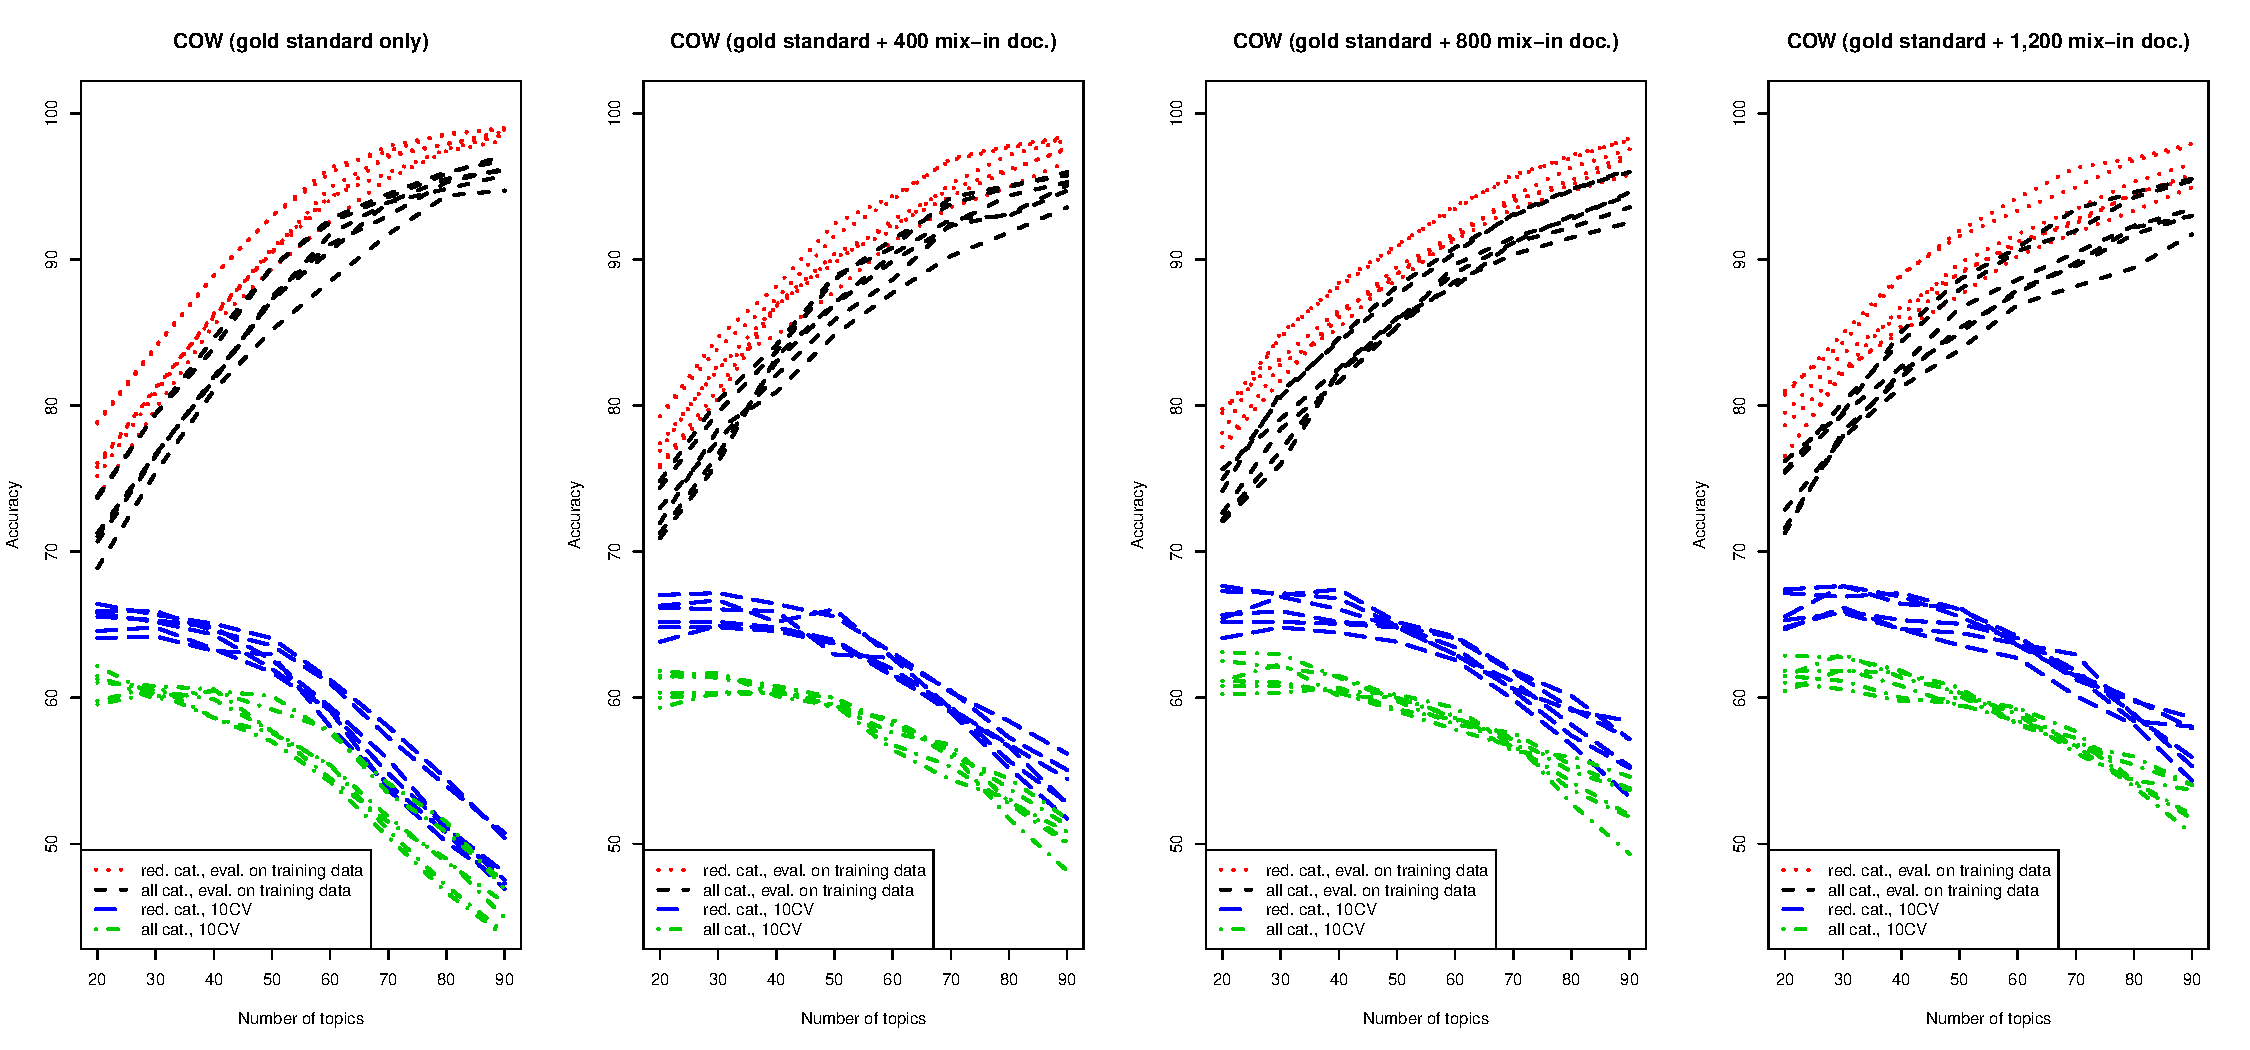
\includegraphics[width=\textwidth]{graphics/cow.pdf}
  \caption{Accuracy with different numbers of topics for COW-only dataset}
  \label{fig:cow}
\end{figure*}

Our general approach was to infer a topic distribution over a corpus (Section~\ref{sec:goldstandard}) using topic modelling algorithms as a first step.
In the second step, we used the resulting document--topic matrix to infer topic domains for the documents from their assignment to the topics.
To achieve this, supervised classifiers were used.
Through permutation of all available classifiers (with the appropriate capabilities) in the Weka toolkit \cite{HallWitten2011}, LM Trees \cite{LandwehrEa2005} and SVMs with a Pearson VII kernel \cite{UstunEa2006} were found to be most accurate.
Due to minimally higher accuracy, SVMs were used in all subsequent experiments.
Because some topic domains occurred only rarely in the gold standard, and we did not expect the classifier to be able to generalize well from just a few instances.
Therefore, we evaluated the results on the \textit{full} data set and a \textit{reduced} data set with rare categories removed.

For the underlying topic inference, we used LSI and LDA as implemented in the Gensim toolkit \cite{RehurekSojka2010}.
The LDA topic distribution in first experiments was highly unstable, and results were generally unusable.
This was probably due to the comparatively small corpora used.
We consequently only report LSI results here and will return to LDA in further experiments.
However, for any topic modelling algorithm, our corpora have to be considered small.
Therefore, we inferred topics not just based on the annotated gold standard data sets, but also on larger datasets which consisted of the gold standard mixed with additional documents from the source corpora.
We systematically increased the number of mixed-in document in increments of roughly half as many documents as contained in the gold standard corpora.

We pre-processed both corpora in exactly the same way (tokenization, lemmatization, POS-tagging, named entity recognition).
Using the lemma and the simplified POS tags (such as \textit{kindergarten\_nn}) as terms in combination with some filters (use only lower-cased purely alphabetic common and proper noun lemmas between 4 and 30 characters long) mostly gave the best results.
%Vocabularies were filtered to contain only terms with a term-document frequency above 2.
%Terms which occurred in more than 50\% of the documents were also removed.
%Preliminary experiments showed that the exact cutoffs were not crucial, however.

\section{Results}
\label{sec:results}

\begin{figure*}[h]
  \centering
  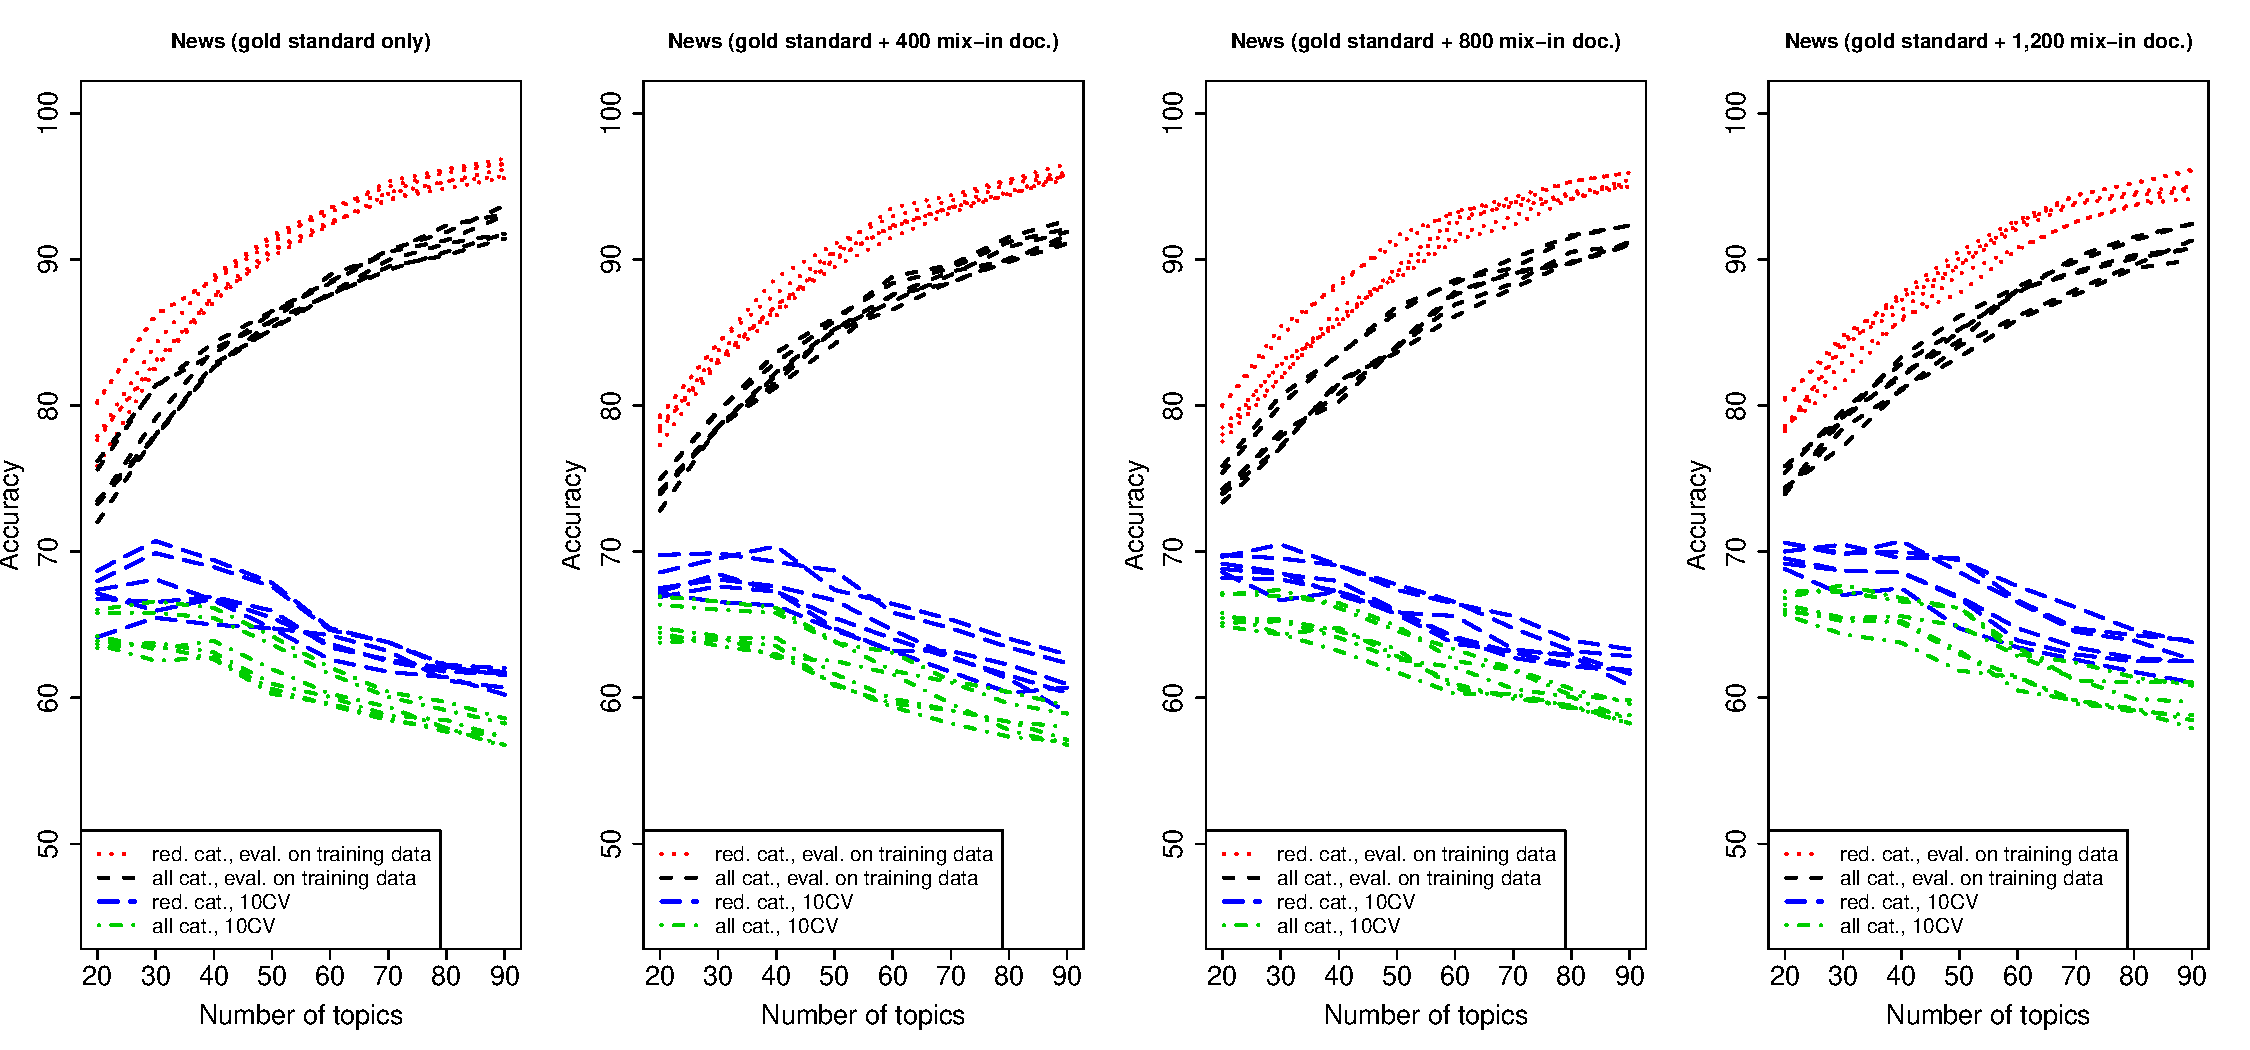
\includegraphics[width=\textwidth]{graphics/dereko.pdf}
  \caption{Accuracy with different numbers of topics for DeReKo-only dataset}
  \label{fig:dereko}
\end{figure*}

\begin{table*}[h]
  \centering
  \resizebox{\textwidth}{!}{\begin{tabular}{|lrllrrrr|}
    \hline
    \textbf{Corpus} & \textbf{Mixed-in} & \textbf{Attribute} & \textbf{Topics} & \textbf{Accuracy} & \textbf{Precision} & \textbf{Recall} & \textbf{F-Measure} \\
    \hline
    COW & $\sim$3,200 & token & 20 & 68.765\% & 0.688 & 0.688 & 0.674 \\
    DeReKo & $\sim$3,600 & lemma + POS & 40 & 72.162\% & 0.716 & 0.722 & 0.686 \\
    COW + DeReKo & 0 & lemma + POS & 30 & 51.872\% & 0.431 & 0.519 & 0.417 \\ 
    \hline
  \end{tabular}}
  \caption{Evaluation at best achievable accuracy with the reduced set of topic domains in 10-fold cross-validation; Precision, Recall, and F-Measure are weighted averages across all categories}
  \label{tab:quality}
\end{table*}

Figure~\ref{fig:cow} shows the classification accuracy using 20 to 90 LSI topics.
Each line corresponds to one sub-experiment (slightly different pre-processing options), and the lines form well distinguishable bands.
The highest accuracy is achieved with the reduced set of topic domains (minor categories removed) when the evaluation is performed on the training data.
The full set of topic domains leads to a drop in accuracy of about 5\%.
The two lower bands show the classification accuracy in a 10-fold cross-validation (10CV), again with the reduced set of topic domains performing roughly 5\% better.
While a higher number of topics improves results on the training data, the accuracy in the cross-validation drops.
Too large numbers of topics obviously allow the method to pick up idiosyncratic features of single documents or very small clusters of documents, leading to extreme overtraining.

The four panels show results based on different topic models.
Panel (a) uses a topic model inferred only from the 870 gold standard documents.
Results in panel (b) through (d) are based on topic models inferred on larger data sets as described in Section~\ref{sec:experiment}.
In the experiment reported in panel (d), for example, 1,200 documents were added to the 870 gold standard documents.
While the results in the 10CV are slightly improved by mixing in more documents, the maximum achieved accuracy does not significantly change.
We continued the experiment (further results not shown here), mixing in up to 8,000 additional documents with no significant change in comparison with panel (d) in Figure~\ref{fig:cow}.
We consider the maximum 10CV accuracy with the reduced set of topic domains most informative w.\,r.\,t.\ the potential quality of the classifier, and we report it in Table~\ref{tab:quality}.

%With regard to linguistic pre-processing, it should be noticed that it affects the results measurably, but not to extreme degrees.
%Using lemma and trunctated POS tags as attributes (such as \textit{kindergarten\_nn}) in combination with our filter set 2 (use only lower-cased purely alphabetic common and proper noun lemmas between 4 and 30 characters long) gave the best results overall.
%The fact that we achieved better performance with non-lower-cased raw tokens on the COW data set (Table~\ref{tab:quality}) shows that differences are marginal, however.

A parallel plot for the DeReKo data is shown in Figure~\ref{fig:coreko}, and maximally best results are also given in Table~\ref{tab:quality}.
The picture is essentially the same as for the COW data set.
The added accuracy (3.397\% according to Table~\ref{tab:quality}) is a side effect of the more skewed distribution of topic domains in the DeReKo gold standard data.
The $\kappa$ statistic for the COW and DeReKo results from Table~\ref{tab:quality} of $\kappa_{\textrm{\tiny COW}}=0.575$ and $\kappa_{\textrm{\tiny DeReKo}}=0.569$ show that achieving a higher accuracy for the COW data is actually harder than with the DeReKo data.

\begin{figure*}[h]
  \centering
  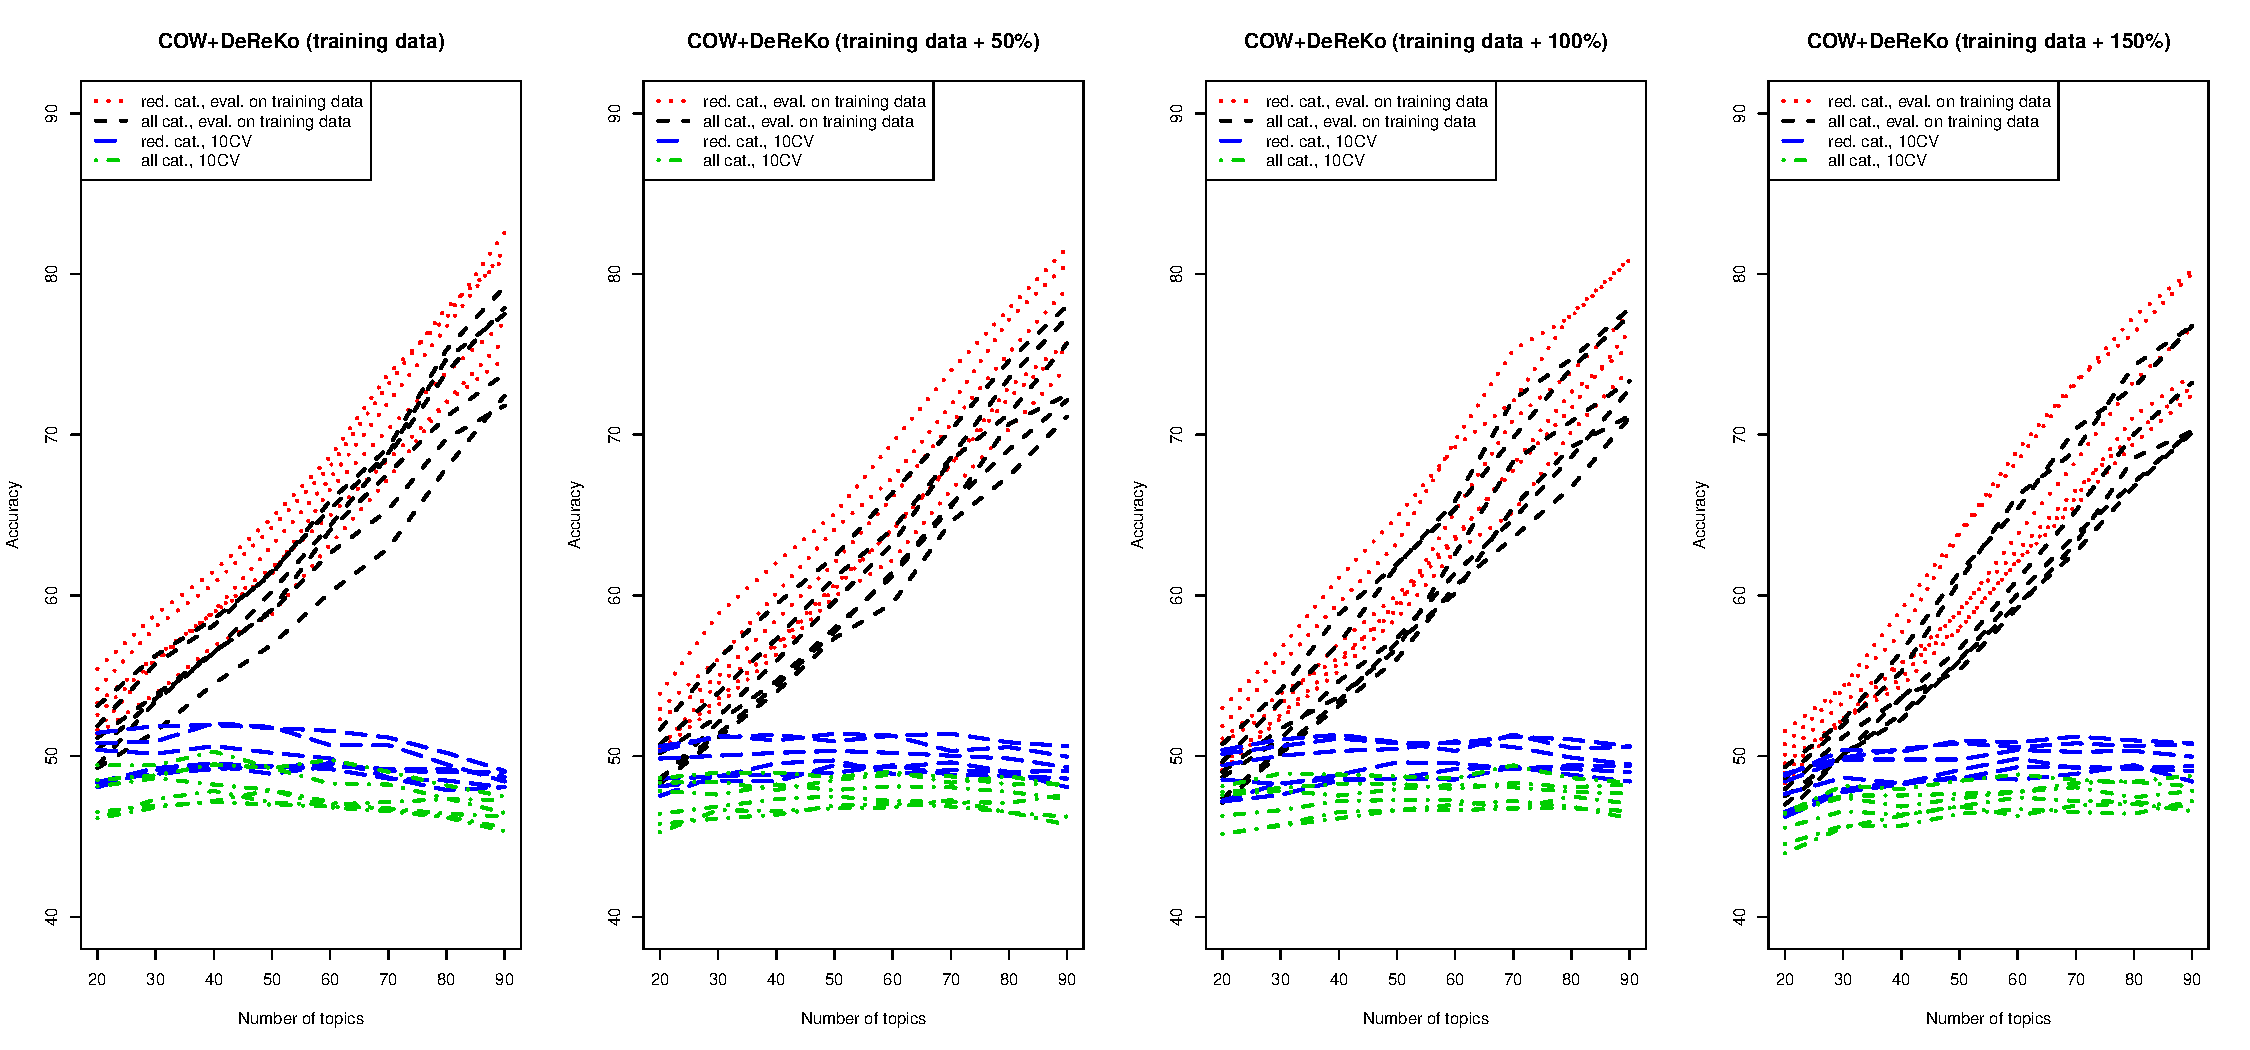
\includegraphics[width=\textwidth]{graphics/coreko.pdf}
  \caption{Accuracy with different numbers of topics for COW+DeReKo dataset}
  \label{fig:coreko}
\end{figure*}

When the COW and DeReKo data are pooled, however, quality drops below any acceptable level, cf.\ Figure~\ref{fig:coreko} and Table~\ref{tab:quality}.
Mixing in more documents improves the evaluation results on the training data, but the 10CV results remains steady at around 50\%.
This is remarkable because larger training data sets should lead to increased, not degraded accuracy.
While a deeper analysis of the LSI topic distributions remains to be undertaken, it is evident what causes these below average results on the side of the SVM classifier when looking at the confusion matrices, cf.\ Table~\ref{tab:confusion}.
The dominant modal category is \textit{Life and Leisure} in the annotated COW gold standard (panel a).
However, the distribution of topic domains is not too skewed, and the confusion is distributed roughly uniformly across categories.
The DeReKo data set (panel b) consists mainly of two clusters of documents in the domains \textit{Politics and Society} (276 of 837) and \textit{Life and Leisure} (350 of 837).
In the joint data set (panel c), this leads to a situation in which the classifier tips over and assigns most documents to \textit{Life and Leisure} and the rest mostly to \textit{Politics and Society}.
This indicates that for such skewed distributions of topic domains, larger gold standard data sets are required.
It is not indicative of a general failure of the method or a general incompatibility of newspaper and web data in the context of our method.
The confusion matrices in Table~\ref{tab:confusion} definitely show, however, that topic domains are represented quite differently in newspaper and web corpora.

\begin{table*}[h]
  \centering
  \resizebox{0.33\textwidth}{!}{\begin{tabular}{|llcccccccc|}
    \hline
    \multicolumn{2}{|c}{\textbf{COW}} & \multicolumn{8}{c|}{\textbf{Classified}} \\
     && \rot{\textbf{PolSoc~}} & \rot{\textbf{Busi}} & \rot{\textbf{Life}} & \rot{\textbf{Arts}} & \rot{\textbf{Public~}} & \rot{\textbf{Law}} & \rot{\textbf{Beliefs~}} & \rot{\textbf{Hist}} \\
   \hline
   \multirow{8}{*}{\rot{\textbf{Annotated}}} & \textbf{PolSoc}  & \textbf{26} &  12 &  10 &   1 &   1 &   0 &   1 &   0 \\ 
     & \textbf{Busi}    &  5 & \textbf{105} &  40 &   7 &   1 &   2 &   1 &   1 \\ 
     & \textbf{Life}    &  3 &  14 & \textbf{286} &   6 &   4 &   1 &   1 &   1 \\ 
     & \textbf{Arts}    &  3 &   2 &  36 &  \textbf{78} &   1 &   0 &   2 &   6 \\ 
     & \textbf{Public}  &  0 &   3 &  11 &   0 &   \textbf{9} &   1 &   0 &   0 \\ 
     & \textbf{Law}     &  3 &   9 &   8 &   0 &   1 &   \textbf{8} &   0 &   0 \\ 
     & \textbf{Beliefs} &  4 &   3 &  11 &   6 &   1 &   0 &  \textbf{30} &   1 \\ 
     & \textbf{Hist}    &  9 &   0 &   9 &   7 &   1 &   1 &   2 &  \textbf{15} \\ 
     \hline
 \end{tabular}}~~\resizebox{0.32\textwidth}{!}{\begin{tabular}{|llcccccccc|}
    \hline
     \multicolumn{2}{|c}{\textbf{DeReKo}} & \multicolumn{8}{c|}{\textbf{Classified}} \\
     && \rot{\textbf{PolSoc~}} & \rot{\textbf{Busi}} & \rot{\textbf{Life}} & \rot{\textbf{Arts}} & \rot{\textbf{Public~}} & \rot{\textbf{Law}} & \rot{\textbf{Beliefs~}} & \rot{\textbf{Hist}} \\
    \hline
    \multirow{8}{*}{\rot{\textbf{Annotated}}} & \textbf{PolSoc}  & \textbf{222} &   5 &  41 &   0 &   8 &   0 &   0 &   0 \\
    & \textbf{Busi}    &  19 &  \textbf{25} &   8 &   0 &   1 &   0 &   0 &   0 \\ 
    & \textbf{Life}    &  27 &   1 & \textbf{321} &   0 &   1 &   0 &   0 &   0 \\ 
    & \textbf{Arts}    &   2 &   0 &  29 &   \textbf{5} &   0 &   0 &   0 &   0 \\ 
    & \textbf{Public}  &  41 &   0 &  27 &   0 &  \textbf{31} &   0 &   0 &   0 \\ 
    & \textbf{Law}     &  10 &   0 &   0 &   0 &   0 &   \textbf{0} &   0 &   0 \\ 
    & \textbf{Beliefs} &   0 &   0 &   3 &   0 &   0 &   0 &   \textbf{0} &   0 \\ 
    & \textbf{Hist}    &   2 &   0 &   7 &   0 &   1 &   0 &   0 &   \textbf{0} \\ 
   \hline
 \end{tabular}}~~\resizebox{0.315\textwidth}{!}{\begin{tabular}{|llccccccccc|}
    \hline
     \multicolumn{2}{|c}{\textbf{Joint}} & \multicolumn{9}{c|}{\textbf{Classified}} \\
     && \rot{\textbf{PolSoc~}} & \rot{\textbf{Busi}} & \rot{\textbf{Medical~}} & \rot{\textbf{Life}} & \rot{\textbf{Arts}} & \rot{\textbf{Public~}} & \rot{\textbf{Law}} & \rot{\textbf{Beliefs~}} & \rot{\textbf{Hist}} \\
    \hline
    \multirow{9}{*}{\rot{\textbf{Annotated}}} & \textbf{PolSoc}   & \textbf{199} &   7 &   0 & 109 &   0 &  12 &   0 &   0 &   0 \\ 
    & \textbf{Busi}     &  18 &  \textbf{23} &   0 & 172 &   0 &   2 &   0 &   0 &   0 \\ 
    & \textbf{Medical}  &   6 &   0 &   \textbf{0} &  29 &   0 &   1 &   0 &   0 &   0 \\ 
    & \textbf{Life}     &  25 &   4 &   0 & \textbf{632} &   0 &   5 &   0 &   0 &   0 \\ 
    & \textbf{Arts}     &   2 &   2 &   0 & 160 &   \textbf{0} &   0 &   0 &   0 &   0 \\ 
    & \textbf{Public}   &  46 &   2 &   0 &  56 &   0 &  \textbf{19} &   0 &   0 &   0 \\ 
    & \textbf{Law}      &   8 &   0 &   0 &  31 &   0 &   0 &   \textbf{0} &   0 &   0 \\ 
    & \textbf{Beliefs}  &   0 &   0 &   0 &  59 &   0 &   0 &   0 &   \textbf{0} &   0 \\ 
    & \textbf{Hist}     &   4 &   0 &   0 &  50 &   0 &   0 &   0 &   0 &   \textbf{0} \\ 
    \hline
 \end{tabular}}
  \caption{Confusion matrices for the best achievable results on the COW (a), DeReKo (b), and joint (c) data sets as reported in Table~\ref{tab:quality}}
  \label{tab:confusion}
\end{table*}

\section{Conclusions and Outlook}
\label{sec:conclusions}

The results presented here are preliminary, but highly encouraging (over 90\% accuracy on training data and over 70\% accuracy in cross-validation on some data sets), and they indicate the route to be taken in further experiments.
First of all, there appears to be a connection between induced topic distributions and more general topic domains.
The decreased performance in cross-validation experiments indicates that larger gold standard data sets are required.
Such data sets are currently being annotated under our supervision.
Secondly, there appears to be a significant difference in the topic distribution and the topic\slash domain mapping in newspaper and web corpora.
This might be one of the reasons behind the collapse of the classifier when newspaper and web data are pooled.
In future experiments, it remains to be discovered whether larger gold standard corpora can alleviate such problems.
This will eventually enable us to decide whether separate models or joint models for the two kinds of corpora are more appropriate.
Thirdly, the highly skewed topic distributions in both newspaper and web data sets indicate that splitting up some topic domains might lead to a better fit.
In fact, annotators have independently asked whether splitting up \textit{Politics and Society} and \textit{Life and Leisure}---the critical categories which make the classifier collapse (cf.\ Section~\ref{sec:results})---could not be split up into at least two categories.

\bibliography{coreko}
\bibliographystyle{acl2016}

\end{document}
